\label{Software architecture views}
\section{Software architecture views}
This chapter discuses the architecture of the system. It is first split into smaller parts and their dependencies on each other. The second paragraph describes the relation between hardware and software is explained. The third paragraph explains the data management. And the fourth paragraph describes the concurrency of the system.

\subsection{Subsystem decomposition}

The component diagram at \textbf{figure~\ref{fig:comp_diag}} shows the relations between the Tygron API, the connector and the GOAL agent. 

\begin{figure}[h]
	  \centering
	  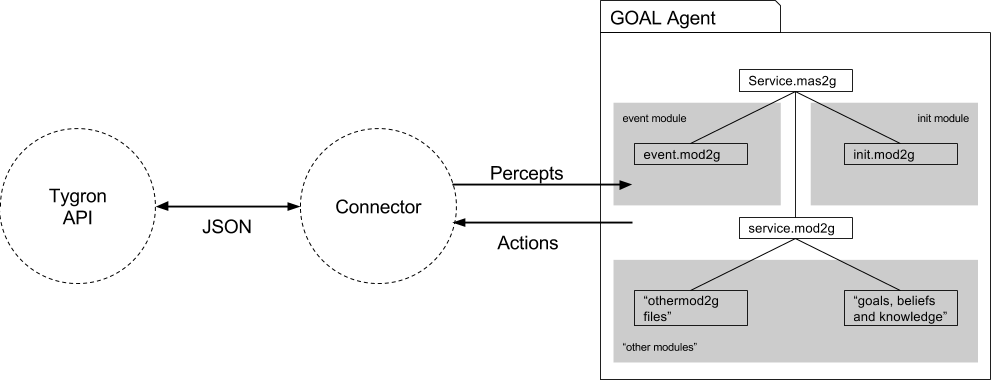
\includegraphics[width=0.7\textwidth]{system_decomposition}
	  \caption{The component diagram}
	  \label{fig:comp_diag}
\end{figure}
This figure shows the different components the project uses and how they connect to each each other. You can see how our bot connects to the connector which in turn will connect to the Tygron API. The Tygron API exists of the module SDK (software development kit) which consists of all the graphics and calculations, basicly the tygron game itself. The Connector uses the environment module, which is everything needed to connect a bot to the game and get and send information from the bot to the game. Finally, the Goal Agent consists of all the modules needed to run the bot.

This starts with the service.mas2g file, which is more or less the main class from which everything happens. This makes use of the init.mod2g file to get all data it needs at the start of the game, and events to get data which is changed, added or removed later in the game. Finally it uses service.mod2g, which handles the main module the bot does. It uses goals, beliefs, and knowledge as data it can use and the other mod.2g as actions it does (for example build.mod2g for building).

\subsection{Hardware/software mapping}
Our virtual human uses a different connection approach to the server than a real human user. When a session is created via the server, a user connects through its own client to that session. \textbf{figure~\ref{fig:Hard_soft_map}} shows that our virtual human will connect to the session using a connector to coneect with the Tygron SDK, which in turn handles the connection to the server. Visualisation of the actions performed by the virtual human are visible through a seperate instance of the Tygron Engine.

\begin{figure}
	\centering
	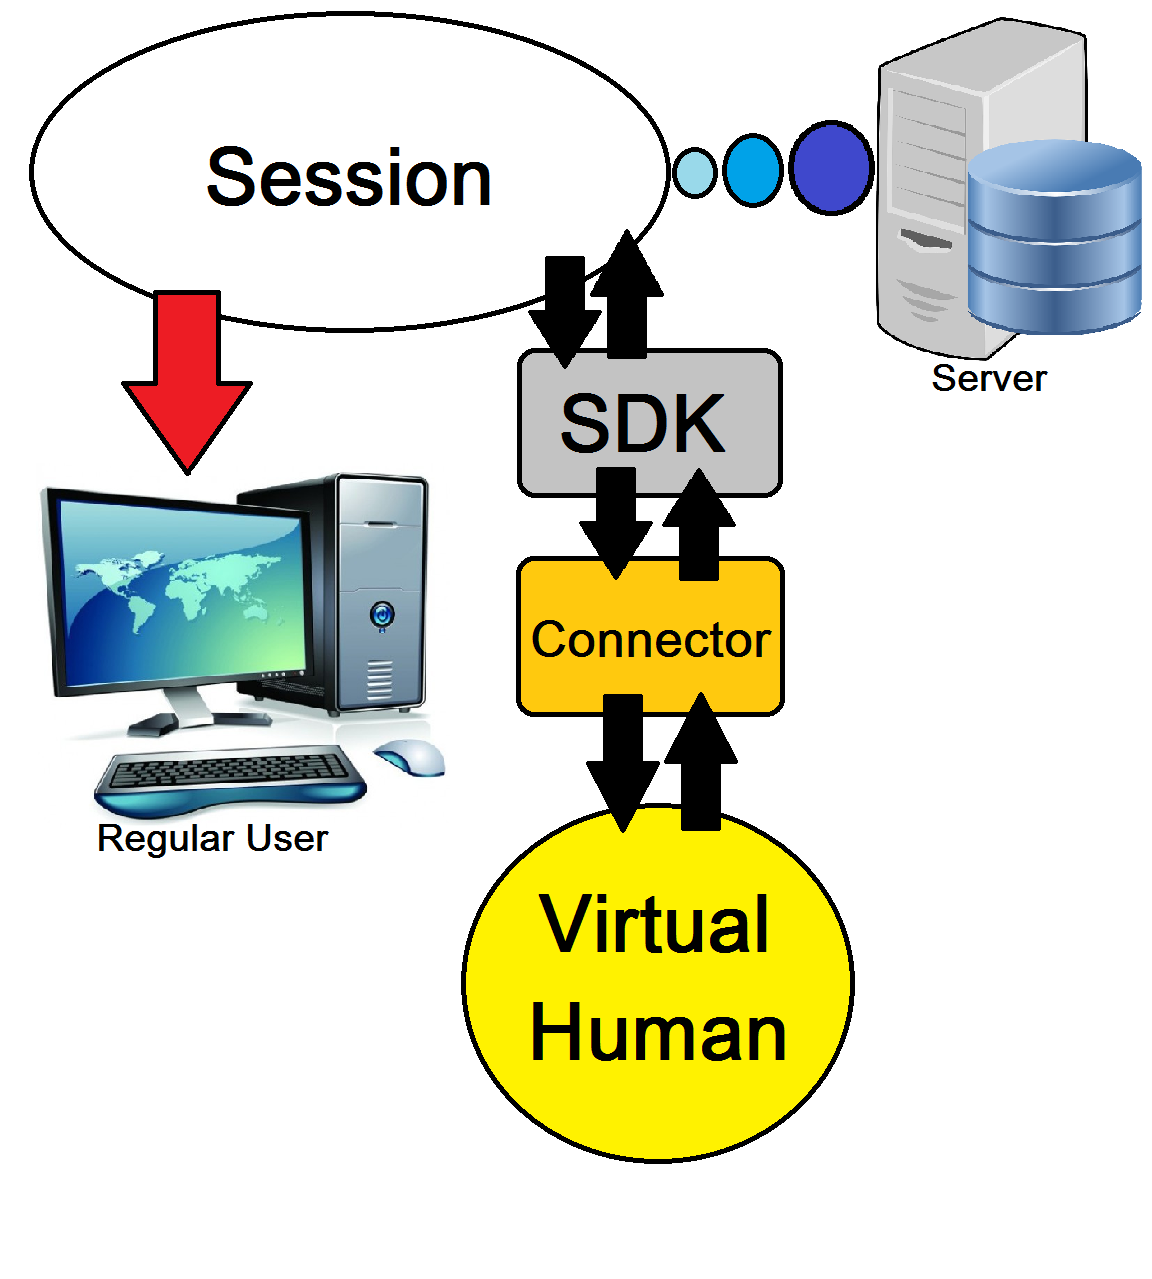
\includegraphics[width=0.5\textwidth]{Hardware_software_mapping}
	\caption{Hardware software mapping}
	\label{fig:Hard_soft_map}
\end{figure}

\subsection{Persistent data management}
When our goal connects to the Tygron engine, the engine loads the game session from its data. Everytime when our bot makes changes in the game, those changes are stored in the engine. Our bot will then read those changes from the engine and choose its next actions, which thereafter will be stored again in the engine. When our bot has reached all its goals, and there are no more updates from the game engine, the data will be kept in the tygron engine. So our GOAL agent is not responsible for storing persistent data and it does not have external files or databases. This is so because just like a regular user would save his progress on the tygron server, our bot will ensure everything is stored on the database of the Tygron server as well.

\subsection{Concurrency}
In the project, the goal agent is dependent on the Tygron engine. This is because the GOAL agent interacts with the tygron engine, so if the engine crashes, or bot will not know what to do anymore either. The connection betweend the Tygron Engine and the Goal Agent is done over the connector, which was partly developed by Tygron and partly by us. The fact that our GOAL agent is dependent on the Tygron engine is something unavoidable, but this causes various problems. The biggest problem is, that for testing the GOAL bot, we also need to use the Tygron engine, and it may happen that the Tygron server which the Tygron engine doesn't work, which then causes the Goal Agent tests to fail. \\
The goal agent shares recourses with other users of the Tygron environment. If a deadlock occurs, this would be on the Tygron environment and not very differently than when a deadlock would occur with human users. That is why our GOAL system won't have issues with deadlocks.
\newpage
